\documentclass[a4]{article}
\usepackage{geometry}
\geometry{verbose,tmargin=2.5cm,bmargin=2.5cm,lmargin=3cm,rmargin=3cm}
\usepackage{amsmath,amssymb,amsthm}
\usepackage{graphicx}
\graphicspath{{graphics/}}
\usepackage[utf8]{inputenc}
\usepackage{fancyvrb}
\usepackage{hyperref}
\usepackage{lscape}
\usepackage{adjustbox}
\usepackage{verbatim}

\title{MultiFEBE \\ ME-TH-SR-001 [TUTORIAL] \\ Cantilever beam (FEM model)}
\author{\'A.G. Vega-Artiles}
\date{September 2022}

\begin{document}

\maketitle

\tableofcontents 

\section{Problem description}

In this fifth tutorial, a static analysis of an elastic straight beam is performed using the Finite Element Method (FEM), i.e. finite elements. Figure \ref{fig:beam} shows the geometry. Required material and geometric properties are the Young's modulus $E$, the Poisson's ratio $\nu$, the density $\rho$, the hysteretic damping $\xi$, the length $L$, the square-shaped cross section $1 \medspace \mathrm{m} \medspace \mathrm{x} \medspace 1 \medspace \mathrm{m}$ and the harmonic force $F$. The force $F$ can be regarded as a P-wave. Self-weight is not considered. 

The natural frequencies to this problem can be obtained by means of the following equations \cite{clough}:

\begin{equation}
	\begin{array}{l}
		\omega_1 = (1.875)^2 \cdot \sqrt{EI /(\overline{m}L^4)} \medspace \mathrm{rad/s} \\
		\omega_2 = (4.694)^2 \cdot \sqrt{EI /(\overline{m}L^4)} \medspace \mathrm{rad/s} \\
		\omega_3 = (7.855)^2 \cdot \sqrt{EI /(\overline{m}L^4)} \medspace \mathrm{rad/s}
	\end{array}
\end{equation}

The problem is solved for $L=10$ $\mathrm{m}$, $E=200\cdot 10^9$ $\mathrm{N/m^2}$, $\nu=0.26$, $\rho=7850$ $\mathrm{kg/m^3}$, mass per unit length $\overline{m}=7850$ $\mathrm{kg/m}$, $\xi=0.02$ and $F=1000$ $\mathrm{N/m^2}$. First, second and third natural frequencies are: 

\begin{equation}
	\begin{array}{l}
		\omega_1 = 51.23 \medspace \mathrm{rad/s} \\
		\omega_2 = 321.05 \medspace \mathrm{rad/s} \\
		\omega_3 = 899.05 \medspace \mathrm{rad/s}
	\end{array}
\end{equation}

\begin{figure}[h!]
	\centering
	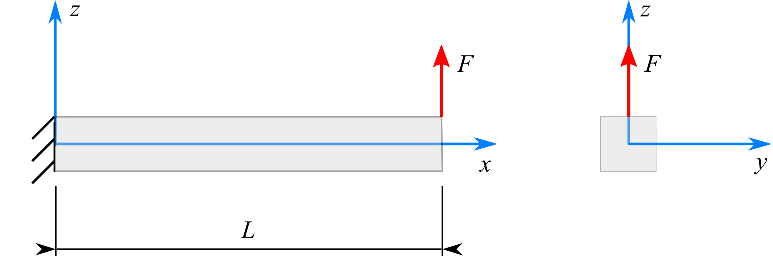
\includegraphics{beam.pdf}
	\caption{Problem layout.}
	\label{fig:beam}
\end{figure}

\section{Pre-processing} 

Pre-processing in MultiFEBE consists of defining the geometry and mesh of the problem. There are three ways to do such definition: directly from the input file (mode = 0), from another file in the native format (mode = 1) or from another file in the Gmsh MSH file format version 2.2 (mode = 2).

\subsection{Gmsh format}

Gmsh \cite{gmsh, gmshweb} is a finite element mesh generator and post-processor with its own language. The software allows to create the geometry in a “bottom-up” manner, going from the most basic elements (points) to the highest order elements (volumes) or in a “Constructive Solid Geometry” manner (boolean operations) or with a combination of methodologies. Gmsh also allows to define the so-called “physical groups” which are ``groups of model entities" that gather elementary entities, where every entity must have a unique tag. On the other hand, the file containing all this geometric definition is the *.geo file whereas the mesh definition is in the *.msh file. 

\subsubsection{GEO file}

The Gmsh language allows to define parameters to use later in the script and comments as every other programming language. In this example two parameters are defined: the square side length (L) and the mesh element size (es). Every point in the geometry can be specified by its coordinates (x y z) and the mesh element size to use there with the function ``Point" and every straight line of the model is created with the function ``Line" and its initial and final points. Then, with the function ``Physical Line" every line is converted into a single entity or physical entity with its own name. Furthermore, it is worth noting that “if an expression defines a new entity, it is enclosed between parentheses but if an expression refers to a previously defined entity, it is enclosed between braces.” \cite{gmshweb} 

Finally, the mesh generation, the element order and the *.msh file saving can also be specified with the expressions ``Mesh + mesh dimension", ``SetOrder + element order" and ``Save + name.msh", respectively.

The resulting *.geo file applied to the problem is the following:

\begin{Verbatim}
// Geometry & mesh parameters
Lbeam = 10;
ms_beam = 2.5;

Point (1) = {0, 0, 0, ms_beam};
Point (2) = {Lbeam, 0, 0, ms_beam};
Line  (1) = {1, 2};
Physical Line ("beam") = {1};

// Mesh generation
Mesh 1;
SetOrder 2;
Save "mesh.msh";
\end{Verbatim}

\subsubsection{MSH file}

The *.msh file begins with a mandatory section about information of the file (MeshFormat) and following by the other sections. Here, three sections are used: the physical group names (PhysicalName), the nodes (Nodes) and the elements (Elements).

In the section ``PhysicalName", all the physical entities of the model are defined. The first line indicates the number of physical entities. Then, one line per physical entity indicating the physical dimension, the tag and the name.  

In the section ``Nodes", all the nodes of the model are defined. The first line indicates the number of nodes. Then, one line per node indicating the node identifier and its coordinates (x y z).

In the section ``Elements", all the elements of the model are defined. The first line indicates the number of elements. Then, one line per element indicating:


\begin{itemize}
	\item Element identifier.
	\item Type of element.
	\item Number of auxiliary tags.
	\item List of tags, where the two first auxiliary tags are mandatory, and the first one corresponds to the identifier of the physical entity to which the element belongs and the second one is the identifier of the elementary model entity to which the element belongs. The rest of the tags are optional.
	\item A list of identifiers corresponding to the nodes of the element.
\end{itemize}

For example, in this case, an element with the identifiers 1 8 2 1 1 1 3 6 corresponds to:

\begin{itemize}
	\item 1: element 1.
	\item 8: type 8 (3-point line).
	\item 2: it has 2 auxiliary tags.
	\item 1: it belongs to the physical entity 1.
	\item 1: it belongs to the line 3.
	\item 1, 3, 6: it connects the nodes 1, 3 and 6.
\end{itemize} 

Finally, the *.msh file can be obtain in  \textit{File $\to$ Export} or by following the instructions specified in the section \textit{GEO file}.

The resulting *.msh file applied to the problem is the following:

\begin{Verbatim}
$MeshFormat
2.2 0 8
$EndMeshFormat

$PhysicalNames
1
1 1 "beam"
$EndPhysicalNames

$Nodes
9
1 0 0 0
2 10 0 0
3 2.499999999995362 0 0
4 4.999999999992398 0 0
5 7.499999999996199 0 0
6 1.249999999998515 0 0
7 3.74999999999364 0 0
8 6.249999999994298 0 0
9 8.749999999998455 0 0
$EndNodes

$Elements
4
1 8 2 1 1 1 3 6
2 8 2 1 1 3 4 7
3 8 2 1 1 4 5 8
4 8 2 1 1 5 2 9
$EndElements
\end{Verbatim}

\subsection{Input data file}
Solving in MultiFEBE consists of running the software by specifying several options in the following sections\footnote{See reference manual.}: [problem], [settings], [materials], [boundaries], [regions] and [conditions over the boundaries].

The first part to configurate is the problem definition in the section [problem]. This example is a 3D harmonic mechanical problem.  

\begin{Verbatim}	
[problem]
type = mechanics
analysis = harmonic
n = 3D
\end{Verbatim}

Then, a list of frequencies is generated by specifying the number of frequencies, that must be $\geq 2$, (10000), followed by the minimum frequency, $>$ 0, ($0.001$) and the maximum frequency ($1000$), being each one in new lines.

\begin{Verbatim}
[frequencies]
rad/s
lin
10000
0.001
1000
\end{Verbatim}

As the problem has just one material, the section [materials] will need two lines: a first line for the number of materials in the model and a second line for the properties such as tag, type, $\rho$, E, $\nu$ and $\xi$.

\begin{Verbatim}
[materials]
1
1 elastic_solid rho 7850. E 200.E9 nu 0.26 xi 0.001
\end{Verbatim}

Next step is to configurate the mesh. In this case, a mesh from Gmsh will be used so that it is necessary to write the option number 2 and the document name obtained from it in the section [settings]. However, if the mesh were going to be read from the input file, it would require to write the sections [nodes], [elements] and [parts] instead.

\begin{Verbatim}	
[settings]
mesh_file_mode = 2 "mesh.msh"
\end{Verbatim}

The section [fe subregions] indicates the number of fe subregions in the first line (1) and a line per subregion indicating the subregion identifier (1) and the part identifier (1). The last two zeros at the end are mandatory and they are going to be used in the future for additional features.

\begin{Verbatim}
[fe subregions]
1
1 1 0 0
\end{Verbatim}

In the section [cross sections], it is necessary to specify the number of cross sections in the first line and a line per cross section by indicating the type of fe (strbeam\_eb = straight beam, Euler–Bernoulli model), number of fe subregions related to the cross section (1), fe subregion identifier (1), type of cross section (rectangle), y dimension (1), z dimension (1), reference vector for y' direction (0. 1. 0.).

\begin{Verbatim}
[cross sections]
1
strbeam_eb 1 1 rectangle 1. 1. 0. 1. 0.
\end{Verbatim}

The format of the  section [regions] consists of a first line indicating the number of regions (1). Furthermore, for each region there must be a block of data consisting of several lines of data. The first one is the region identifier and the region class (discretization method) (1 fe). As the region is a FE region, then the second line indicates the number of subregions (1) and their identifiers (1).

\begin{Verbatim}	
[regions]
1
1 fe
1 1
material 1
\end{Verbatim}

In the section [groups], nodes and elements can be tagged depending on the chosen option. The first line indicates the number of groups and then a line per group with the group tag and the command. In this example, only one group is created with all the elements. 

\begin{Verbatim}
[groups]
1
1 elements all
\end{Verbatim}

In the section [element options], several options can be set in elements. In this example, the mid-nodes of the elements tagged as group 1 are set to be shown in the resulting files.  

\begin{Verbatim}
[element options]
group 1 strbeam_line3_midnode_rotation 1
\end{Verbatim}

In the section [conditions over nodes], all boundary conditions over nodes will be specified. For 3D finite element nodes, after ``node id:" there are 6 lines, where the first one indicates the node where the boundary condition is assigned as ``node id:", followed by a pair of values indicating the type and value of the boundary condition for each traslation direction x, y and z, and rotation axis x, y and z, being each one in a new line. The first value indicates the type of boundary condition (0 for prescribed displacement/rotation and 1 for prescribed force/moment) and the second one the value of the boundary condition as a complex number (real part, imaginary part) because it is a harmonic analysis. 

\begin{Verbatim}	
[conditions over nodes]
node 1: 0 (0.,0.)
        0 (0.,0.)
        0 (0.,0.)
        0 (0.,0.)
        0 (0.,0.)
        0 (0.,0.)

node 2: 1 (0.,0.)
        1 (0.,0.)
        1 (1000.,0.)
        1 (0.,0.)
        1 (0.,0.)
        1 (0.,0.)
\end{Verbatim}

The whole data file applied to the problem is the following:

\begin{Verbatim}
[problem]
type = mechanics
analysis = harmonic
n = 3D

[frequencies]
rad/s
lin
10000
0.001
1000

[materials]
1
1 elastic_solid rho 7850. E 200.E9 nu 0.26 xi 0.001

[settings]
mesh_file_mode = 2 "mesh.msh"

[fe subregions]
1
1 1 0 0

[cross sections]
1
strbeam_eb 1 1 rectangle 1. 1. 0. 1. 0.

[regions]
1
1 fe
1 1
material 1

[groups]
1
1 elements all

[element options]
group 1 strbeam_line3_midnode_rotation 1

[conditions over nodes]
node 1: 0 (0.,0.)
        0 (0.,0.)
        0 (0.,0.)
        0 (0.,0.)
        0 (0.,0.)
        0 (0.,0.)

node 2: 1 (0.,0.)
        1 (0.,0.)
        1 (1000.,0.)
        1 (0.,0.)
        1 (0.,0.)
        1 (0.,0.)
\end{Verbatim}

\section{Results and discussion}

The results of the node 2 (pile head) were taken and plotted together with the analytical solution to observe the frequency response in Figure \ref{fig:beam_results}. The option by default in MultiFEBE adds the rotational inertia of the beam cross section (Rayleigh beam) \cite{han}, but this effect is not included in Clough \cite{clough}. This is the reason for the discrepancy between the numerical and analytical solution. However, this contribution can be deactivated by going to ``MultiFEBE/lib/fbem/src/fem\_beams.f90", suppressing ``Mr" in the function ``fbem\_fem\_strbeam\_Ml (line 1339) and recompiling.

The results without the effect of rotational inertia of the beam cross-section are also shown in Figure \ref{fig:beam_results}. In this case, it can be seen that the numerical solution is in perfect agreement with the analytical solution.

\begin{figure}[h]
	\centering
	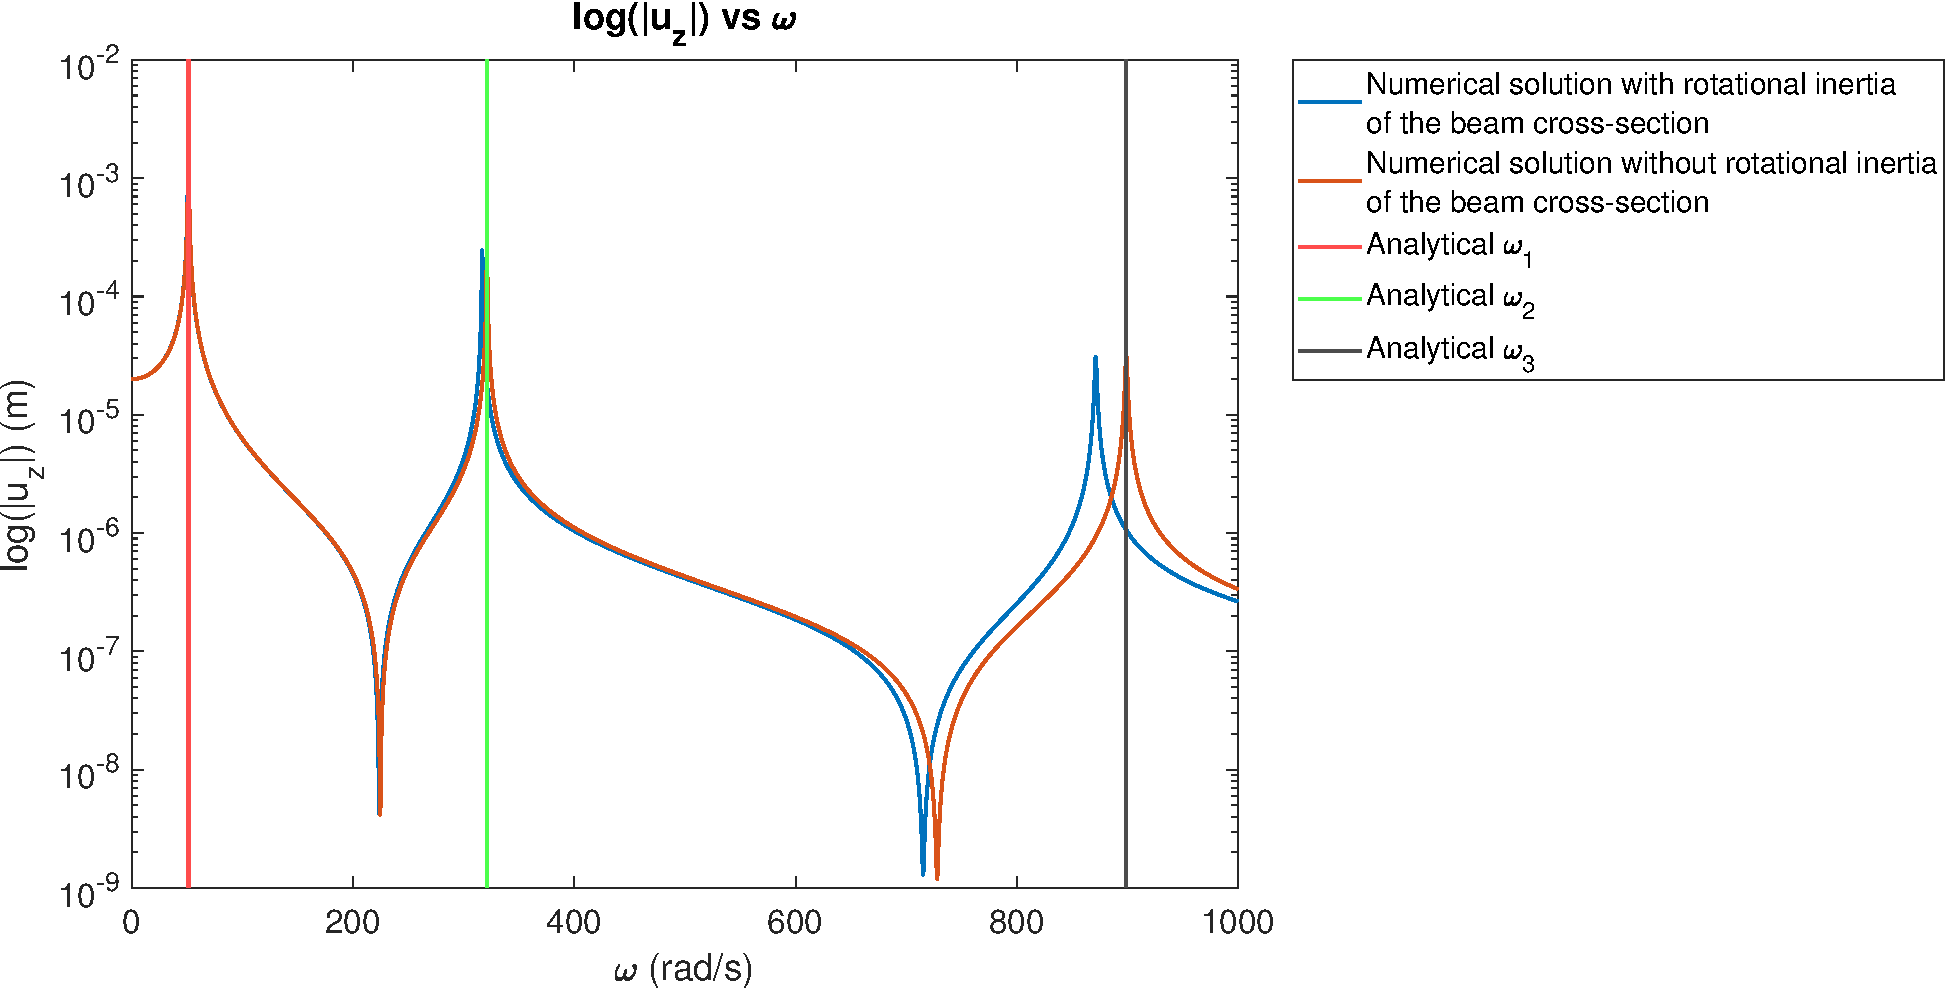
\includegraphics[scale = 0.45]{uz_vs_w.pdf}
	\caption{Results of the harmonic straight beam.}
	\label{fig:beam_results}
\end{figure}

\begin{thebibliography}{99}
	
	\bibitem{clough} R. W. Clough and J. Penzien. ``Dynamics of structures." \textit{Computers \& Structures. Inc.}, (2003).
	
	\bibitem{gmsh} C. Geuzaine and J.-F. Remacle, ``Gmsh: a three-dimensional finite element mesh generator with built-in pre- and post-processing facilities." \textit{International Journal for Numerical Methods in Engineering}, Volume 79, Issue 11, pages 1309--1331, (2009).
	
	\bibitem{gmshweb}  C. Geuzaine and J.-F. Remacle, ``Gmsh." \url{http://gmsh.info/}
	
	\bibitem{han} S. M. Han, H. Benaroya and T. Wei. ``Dynamics of transversely vibrating beams using four engineering theories." \textit{Journal of Sound and vibration}, Volume 225, Issue 5, pages 935--988, (1999).
	
\end{thebibliography}

\end{document}
